\documentclass[a4paper,norsk, 10pt]{article}
\usepackage[utf8]{inputenc}
\usepackage{verbatim}
\usepackage{listings}
\usepackage{graphicx}
\usepackage[norsk]{babel}
\usepackage{a4wide}
\usepackage{color}
\usepackage{amsmath}
\usepackage{float}
\usepackage{amssymb}
\usepackage[dvips]{epsfig}
\usepackage[toc,page]{appendix}
\usepackage[T1]{fontenc}
\usepackage{cite} % [2,3,4] --> [2--4]
\usepackage{shadow}
\usepackage{hyperref}
\usepackage{titling}
\usepackage{marvosym }
\usepackage{subcaption}
\usepackage[noabbrev]{cleveref}
\usepackage{cite}


\setlength{\droptitle}{-10em}   % This is your set screw

\setcounter{tocdepth}{2}

\lstset{language=c++}
\lstset{alsolanguage=[90]Fortran}
\lstset{alsolanguage=Python}
\lstset{basicstyle=\small}
\lstset{backgroundcolor=\color{white}}
\lstset{frame=single}
\lstset{stringstyle=\ttfamily}
\lstset{keywordstyle=\color{red}\bfseries}
\lstset{commentstyle=\itshape\color{blue}}
\lstset{showspaces=false}
\lstset{showstringspaces=false}
\lstset{showtabs=false}
\lstset{breaklines}
\title{FYS3140 Oblig1}
\author{Daniel Heinesen, daniehei}
\begin{document}
\maketitle

\section*{1)}
\subsection*{a)}

A block is sliding on a surface, connected with a spring, with a pendulum hanging below. Since the block is only moving on the surface, its movement is limited to the x-axis, thus giving us the first constraint. The distance between the block and the pendulum is always constant. This is the second constraint of the system. Since the system is in 2 dimensions, we are going to have

$$
d = 2N - M = 2*2 -2 = 2
$$

generalized coordinates. The only independent coordinates are the position of the block along the x-axis, and the angle of the pendulum. So the generalized coordinates are $x$ and $\theta$.

\subsection*{b)}
For this system we can look at attachment point of the pendulum as one particle and the pendulum as an other. But the position of the attachment point is determent only by $\omega$ and is therefor not a variable, or we can say that the position, both $x$ and $y$, of this point is constrained. The other constraint is that the distance between this point and the pendulum is constant. So the dimension of the configuration space is

$$d = 2N -M = 4 - 3 = 1$$

So the only generalized coordinate we need to describe this system is the angle between the pendulum and the y-axis, $\theta$.

\subsection*{c)}

Here we have 2 bodies, the cylinder and the plank. The cylinder is constrained in that it can only move along the x-axis. The position of the plank is constrained in its movement by the cylinder. It is only capable of rolling on the top of the cylinder. We therefor have that

$$
d = 2N - M = 4 - 2 = 2
$$

I am going to chose the x-position of the cylinder, and the angle between the vector from the center of mass of the cylinder and that of the plank, and the y-axis, $\theta$, as the two generalized coordinates.

\subsection*{d)}

I am not completely sure about the following:\\

There is one constraint in the spinning top, that the distance from the center of mass to the point where the spinning top meets the floor is constant. Standing still we need 3 coordinates to describe the spinning top: pitch-, roll- and yaw angle. But since it can move along the surface, I think we have to have 2 more coordinate, $x$ and $y$, to describe the position of the point where the spinning top meat the floor(the point at which the spinning top rolls and pitches). This gives us a total of 5 coordinates.

\section*{2)}

Looking at the Atwood machine we can view it as a one dimensional system, since the parts only can move up or down. I am going to call the position of mass 1 as $x_1$, mass 2 as $x_2$, mass 3 as $x_3$ and the position of the lower pulley $x_p$. To make the writing easier, I am going to let the axis point downward.\\

There are going to be 2 constraints. The first is that the maximum length between $x_1$ and $x_p$ is going to be the length of the rope, so:

$$
x_p + x_1 = l_1
$$

The same is going to be true for for $x_2$ and $x_3$. But we have to be more careful since we aren't measuring there position for $x=0$. I will instead say that the position $x_3$ is going to be $x_p$ i addition of the rope between mass 3 and the pulley. This gives us:

$$
x_3 = x_p + (l_2 -(x_2 - x_p))
$$

We can see that 

$$ d = 4-M = 4-2 = 2$$

I am therefor going to chose $x_p$ and the distance between $x_p$ and $x_3$, let us call this $x'$ as the generalized coordinates. So we can then write all the coordinates as functions of the generalized coordinates:

$$
x_p = x_p
$$
$$
x_1 = l_1 - x_p
$$
$$
x_2 = x_p + l_2 - x'
$$
$$
x_3 = x_p + x'
$$

We then have to find the velocities:

$$
\dot{x_p} = \dot{x_p}
$$
$$
\dot{x_1} = -\dot{x_p}
$$
$$
\dot{x_2} = \dot{x_p} - \dot{x'}
$$
$$
\dot{x_3} = \dot{x_p} + \dot{x'}
$$

We can now find the energies(notice that both the kinetic and potential energy of the pulley is 0 since it does not have any mass):

$$
T = \frac{1}{2}(m_1\dot{x_1}^2 + m_2\dot{x_2}^2 + m_3\dot{x_3}^2) = -2m\dot{x_p}^2 + m(\dot{x_p} - \dot{x'})^2 + \frac{1}{2}m(\dot{x_p} + \dot{x'})^2
$$

$$
V = -g(m_1x_1 + m_2x_2 + m_3x_3 = -g(4m(l_1 - x_p) + 2m(x_p + l_2 - x') + m(x_p + x') 
$$
$$
= -gm(4l_1 +2l_2 - x_p -x') 
$$

So the Lagrangian is given as

$$
\mathcal{L} = K - V = -2m\dot{x_p}^2 + m(\dot{x_p} - \dot{x'})^2 + \frac{1}{2}m(\dot{x_p} + \dot{x'})^2 + gm(4l_1 +2l_2 - x_p -x') 
$$

\section*{3)}

The constraint of this system is that rods are connected, first by the 2 lower joints, and secondly the two in the ceiling. Since the ceiling isn't moving the rods cannot move anywhere other then around the ceiling joints. This adds up to 5 constraints. Giving us:

$$
d = 3 -2 = 1
$$

We are therefor choosing $\theta$ as the generalized coordinate.\\

We can now look at the energies. First the kinetic energy. The vertical rods are rotating around pivots, giving them the kinetic energy:

$$
K = \frac{1}{2}I\omega^2 = \frac{1}{2}\frac{1}{3}ml^2\dot{\theta}^2
$$

The last, horizontal rod does not rotate. Since the rod is rigid and always laying in horizontally, every point have the same velocity. We can there for look at the velocity of the end point to find the kinetic energy:

$$
K = \frac{1}{2}mv^2 = \frac{1}{2}ml^2\dot{\theta}^2
$$

Giving us a total kinetic energy:

$$
T = 2\cdot \frac{1}{6}ml^2\dot{\theta}^2 + \frac{1}{2}ml^2\dot{\theta}^2 = \frac{5}{6}ml^2\dot{\theta}^2
$$

For the potential energy: the center of mass of the vertical rods have the position $ h = \frac{l}{s}\cos\theta$, while for the horizontal rod $h = l\cos\theta$, so

$$
V = mgh = mg(\frac{l}{s}\cos\theta + \frac{l}{s}\cos\theta + l\cos\theta = 2mgl\cos\theta
$$

Giving us the Lagrangian

$$
\mathcal{L} = T - V = \frac{5}{6}ml^2\dot{\theta}^2 - 2mgl\cos\theta
$$

\section*{4)}
\subsection*{a)}
This system has one particle, and one constraint, namely that $e^{-(x^2 + y^2)} + z = 0$. Therefor:

$$
d = 3N -M = 3 -1 = 2
$$

I therefor chose $x$ and $y$ as the generalized coordinates, and can write the position as:

$$
\vec{r} = x\hat{i} + y\hat{j} - e^{-(x^2 + y^2)}\hat{k}
$$

\subsection*{b)}
A virtual displacement is given by

$$
\delta \vec{r_i} = \sum_{j=1}^d \frac{\partial \vec{r_i}}{\partial q_j} \delta q_j
$$

So

$$
\delta\vec{r_x} = \frac{\partial \vec{r_x}}{\partial x} \delta x = \delta x 
$$
$$
\delta\vec{r_y} = \frac{\partial \vec{r_y}}{\partial y} \delta y = \delta y 
$$
$$
\delta \vec{r_z} = \sum_j \frac{\partial \vec{r_y}}{\partial q_j} \delta q_j = 2xe^{-(x^2 + y^2)} \delta x + 2y e^{-(x^2 + y^2)}\delta y
$$

So

$$
\delta \vec{r} = \delta x \hat{i} + \delta y \hat{j} + 2e^{-(x^2 + y^2)}(\delta x + \delta y)\hat{k}
$$

\subsection*{c)}
To find a vector $\vec{f}$ normal to $\delta \vec{r}$ we are going to use the fact that $\delta \vec{r}$ is tangent to the constraint function. And to find a vector normal to this function we have to take the gradient. So

$$
\vec{f} = \varpropto \nabla (z+e^{-(x^2 + y^2)}) = -2x e^{-(x^2 + y^2)} \hat{i} - 2y e^{-(x^2 + y^2)} \hat{j} + 1
$$

We can check this by

$$
\vec{f} \cdot \delta \vec{r} = -2x e^{-(x^2 + y^2)} \delta x - 2y e^{-(x^2 + y^2)} \delta y + 2e^{-(x^2 + y^2)}(\delta x + \delta y) = 0
$$

This vector will not have the same length, be we have found a vector pointing in the same direction as $\vec{f}$.

\subsection*{d)}
\begin{figure}[H]
\centering
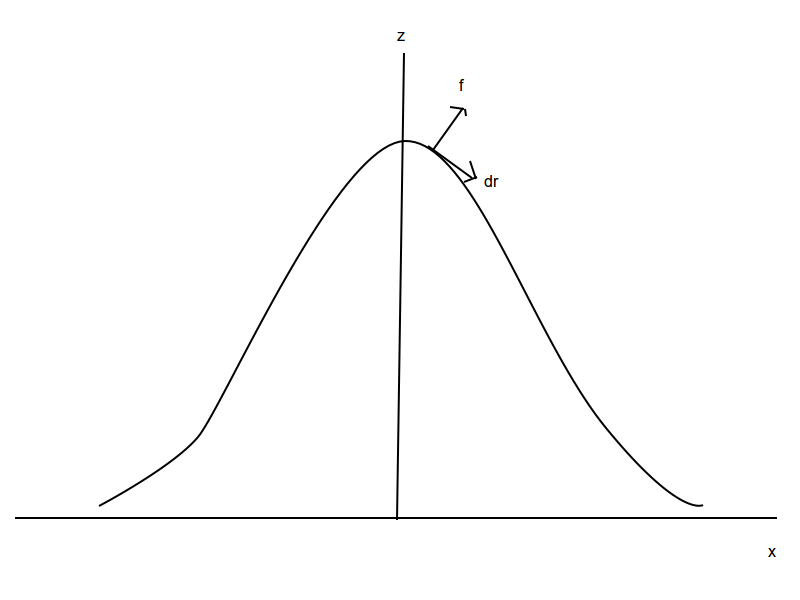
\includegraphics[scale=.4]{4d.png}
\caption{The surface for y=0. We can see that $\delta \vec{r}$ is tangent to the surface ('dr' in the figure.) While $\vec{f}$ is normal to the surface.}
\end{figure}

\section*{4)}
We are going to use the principle of virtual work and that for a system in equilibrium $\mathcal{F_j} = \frac{\partial V}{\partial q_j} = 0$. Because of the constraint that the chain has to be on the surface, we only have 1 coordinate.\\

We are going to 'cheat' somewhat by writing $\frac{\partial V}{\partial q_j} = \frac{\Delta V}{\Delta q_j} = 0$

$$
\delta w = \mathcal{F}\delta q = \frac{\Delta V}{\Delta q} \delta q = \Delta V = 0
$$

Since we are working with a chain, all the parts are dragging each other. By moving one, the next in line will take its place. The only place in the chain where this is not the case is the ends. So we have to look at the potential at the ends. We are moving a little bit in the direction $\delta q$, but we are go to use that over this small displacement, the hight $z$ stays the same. So

$$
\Delta V = V_A - V_B = z_A g\delta m  \delta q  - z_B g\delta m \delta q= 0
$$

This lead us to that

$$
z_A = z_B
$$






\end{document}


